% $File: expr.tex
% $Date: Sun Dec 14 00:25:54 2014 +0800
% $Author: jiakai <jia.kai66@gmail.com>

\section{实验设计及实验结果}
关于卷帘快门的参数测量已在\secref{rolling-shutter}中描述,在此不再赘述。

\subsection{基于合成全局快门数据的全局运动分析\label{sec:synth-global}}
% f{{{
使用如下公式合成可控位移的图像,其效果如\figref{synthesis}所示:
\begin{equation}
    f(x, y) = \sin(\omega_x (x + \delta_x)) + \sin(\omega_y y) + 
    \mathcal{N}(0, \sigma^2)
    \label{eqn:synth-global}
\end{equation}
其中$\delta_x$控制位移,$\sigma$控制噪声,$f(x, y)$被量化到$[0, 255]$间的整数。
\begin{figure}[h!]\begin{center}
    \begin{subfigure}[b]{.35\figwidth}
        \centering
        
\includegraphics[width=.35\figwidth]{res/synth0.png}
    \end{subfigure}
    \begin{subfigure}[b]{.35\figwidth}
        \centering
        \includegraphics[width=.35\figwidth]{res/synth1.png}
    \end{subfigure}
    \caption{合成数据,$\delta_x = 0.01$pxl, $\sigma = 1.35/255$}
    \label{fig:synthesis}
\end{center}\end{figure}

控制$\delta_x$取不同的值,按上述方法得到的相位差如\figref{synthesis:pd}所示。
\begin{figure}[h!]\begin{center}
    \includegraphics[width=.5\figwidth]{res/synth-pd.png}
    \caption{位移与相位差的关系}
    \label{fig:synthesis:pd}
\end{center}\end{figure}

总的来说,基于合成数据的实验证明了之前想法的可行性,
显示相位差与实际位移线性相关,而且对噪声比较鲁棒,
在$\sigma \le 3/255$时都比较有效,已经远低于一般设备的噪声;
但在$\sigma=0$时出现了较大波动,猜测这是由于量化时取整带来的bias造成的,
而在有噪声时可一定程度上抵消这种bias。而为何在噪声太大时由正相关变成了反相关,
我还没有明确的解释。

% f}}}

\subsection{基于实际数据的全局运动分析与低频信号恢复\label{sec:data-global}}
% f{{{

把坐标纸贴在扬声器的震膜上直接拍摄,用扬声器播放10hz, 15hz, 20hz, 25hz的声音,
用Pentax K-01相机拍摄,快门速度为1/2000, iso100, F/5.6, 55mm, 视频为1280x720,
59.940fps, H.264编码。

使用上述方法估计全局运动并直接作为采样信号进行FFT,
发现对单频音和多频音均能较好恢复,
多频音的结果如\figref{real:lowfreq}所示。
\begin{figure}[h!]\begin{center}
    \begin{subfigure}[b]{.5\figwidth}
        \includegraphics[width=.5\figwidth]{res/setting.png}
        \caption{实际拍摄情况}
    \end{subfigure}
    \begin{subfigure}[b]{.5\figwidth}
        \includegraphics[width=.5\figwidth]{res/global-recon.png}
        \caption{重建结果,可见对各频率均能较好恢复;
            其中后半部分的振幅偏高是由于拍摄时误碰了实验装置造成整体位移,
            但对结果影响不大}
    \end{subfigure}
    \caption{基于全局运动分析的低频信号重建}
    \label{fig:real:lowfreq}
\end{center}\end{figure}

% f}}}

\subsection{基于合成卷帘快门数据的局部运动分析\label{sec:synth-local}}
% f{{{
与\secref{synth-global}类似,我们先用合成数据的方法测试算法的可行性。
对\eqnref{synth-global}进行修改,我们使用如下方法合成一段视频,对于第$i$帧:
\begin{eqnarray}
    f(i, x, y) &=& \sin(\omega_x (x + \delta_x(i, y))) + \sin(\omega_y y) + 
    \mathcal{N}(0, \sigma^2) \\
    \delta_x(i, y) &=& A\sin(2\pi f_s(it_f+yd))
    \label{eqn:synth-local}
\end{eqnarray}
实验中,在\eqnref{synth-local}里我们取$A=0.01$表示震动造成的水平位移为$0.01$像素,
$t_f=\frac{1}{60}$为视频每帧的时长,$d=1.57e-5$为线延迟,$f_s=500$为震动频率,
另外$f(i, x, y)$量化到$[0, 255]$间的整数并加上方差为1的白噪声。
另外我们还选取了$f_s=\{500, 800\},\,A=\{0.01, 0.005\}$进行多频音的测试。
对视频前10帧用\secref{algo-hf}所述的方法进行频谱恢复,
结果如\figref{synth-local}所示,
可见在噪声存在的情况下,
该方法能较为准确的恢复卷帘快门成像所包含的高频运动信息。
\begin{figure}[h!]\begin{center}
    \begin{subfigure}[b]{.5\figwidth}
        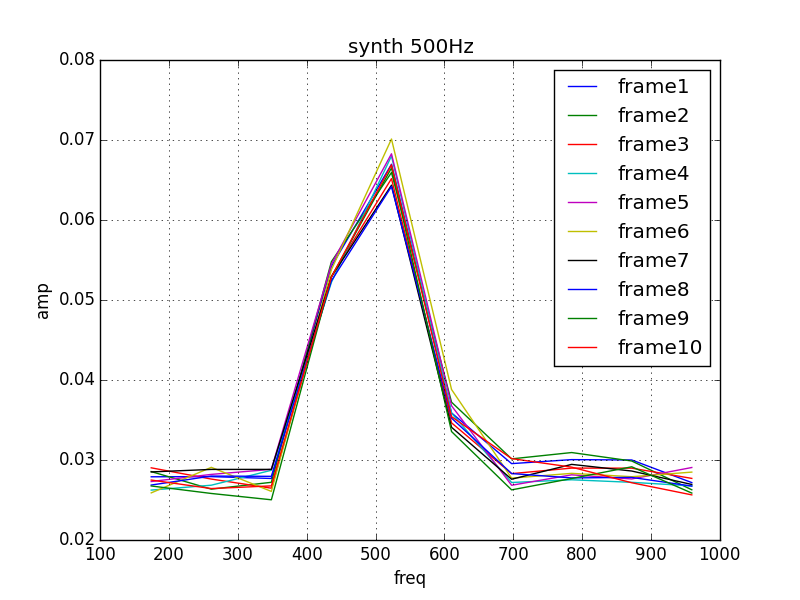
\includegraphics[width=.5\figwidth]{res/synth-500.png}
        \caption{500Hz合成数据的恢复}
    \end{subfigure}
    \begin{subfigure}[b]{.5\figwidth}
        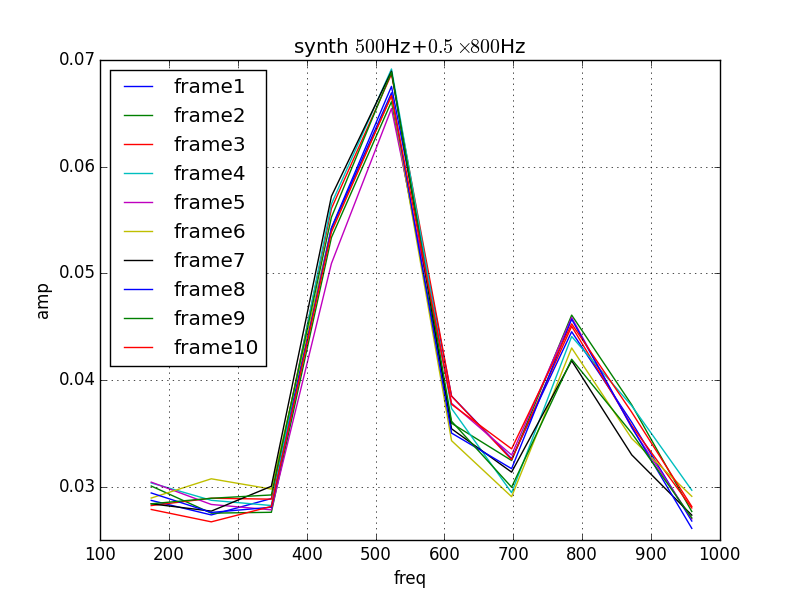
\includegraphics[width=.5\figwidth]{res/synth-500+800.png}
        \caption{500Hz和800Hz,振幅$2:1$合成数据的恢复}
        \label{fig:synth:500+800}
    \end{subfigure}
    \caption{对合成的卷帘快门视频进行频谱分析的结果}
    \label{fig:synth-local}
\end{center}\end{figure}
% f}}}

\subsection{基于实际数据的局部运动分析与高频信号恢复}
与\secref{data-global}采用相同的相机配置,如\secref{algo-hf}所述取
$\theta_m=2$,此时采样率上限为
$\frac{1}{d2^{\theta_m}} \approx 16000$Hz,
而实际可用的采样频率受限于快门速度,不超过$2000$Hz。

我们对单频和双频音进行了测试,发现单频音恢复效果总体不错,
但双频音则效果很差。具体如\figref{real:highfreq}所示。
\begin{figure}[h!]\begin{center}
    \begin{subfigure}[b]{.33\figwidth}
        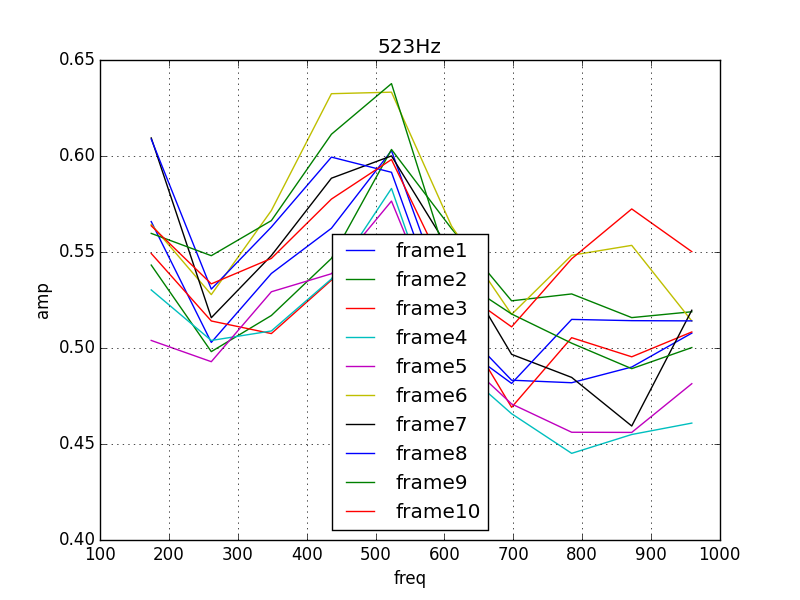
\includegraphics[width=.4\figwidth]{res/data-523.png}
        \caption{$\text{C}_5$(523Hz)单频音的恢复}
    \end{subfigure}
    \begin{subfigure}[b]{.33\figwidth}
        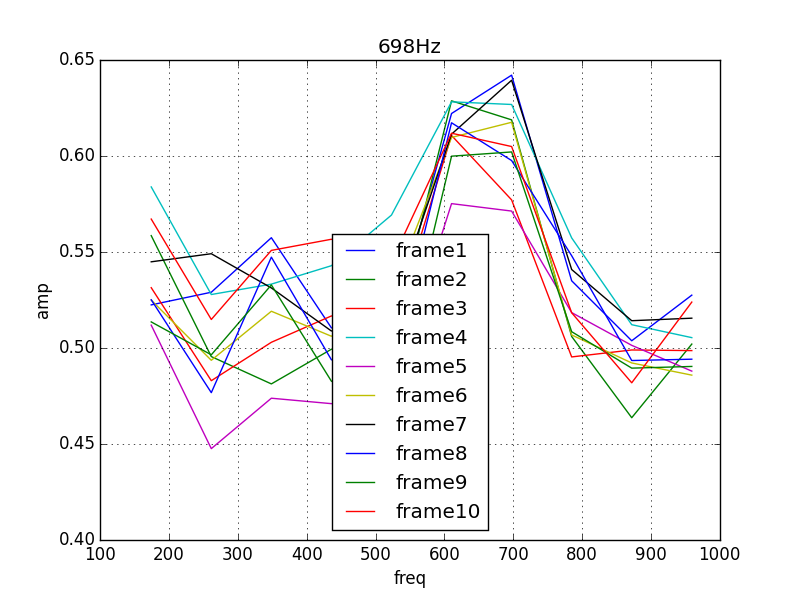
\includegraphics[width=.4\figwidth]{res/data-698.png}
        \caption{$\text{F}_5$(698Hz)单频音的恢复}
    \end{subfigure}
    \begin{subfigure}[b]{.33\figwidth}
        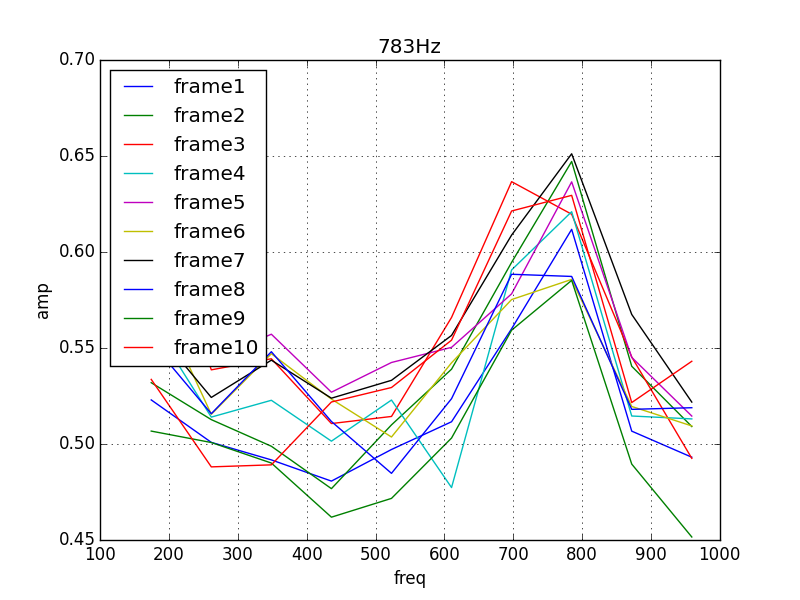
\includegraphics[width=.4\figwidth]{res/data-783.png}
        \caption{$\text{G}_5$(783Hz)单频音的恢复}
    \end{subfigure}
    \begin{subfigure}[b]{.4\figwidth}
        \includegraphics[width=.4\figwidth]{res/data-300+500.png}
        \caption{等幅300Hz+500Hz双频音的恢复}
        \label{fig:real:300+500}
    \end{subfigure}
    \begin{subfigure}[b]{.4\figwidth}
        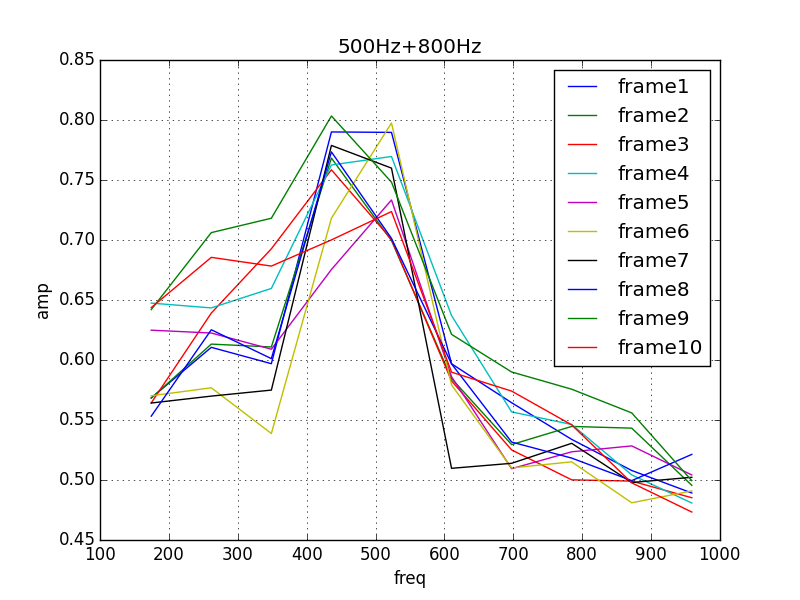
\includegraphics[width=.4\figwidth]{res/data-500+800.png}
        \caption{等幅500Hz+800Hz双频音的恢复}
    \end{subfigure}
    \caption{对实际拍摄视频进行频谱分析的结果}
    \label{fig:real:highfreq}
\end{center}\end{figure}

% vim: filetype=tex foldmethod=marker foldmarker=f{{{,f}}} 
